% Options for packages loaded elsewhere
\PassOptionsToPackage{unicode}{hyperref}
\PassOptionsToPackage{hyphens}{url}
%
\documentclass[
  ignorenonframetext,
]{beamer}
\usepackage{pgfpages}
\setbeamertemplate{caption}[numbered]
\setbeamertemplate{caption label separator}{: }
\setbeamercolor{caption name}{fg=normal text.fg}
\beamertemplatenavigationsymbolsempty
% Prevent slide breaks in the middle of a paragraph
\widowpenalties 1 10000
\raggedbottom
\setbeamertemplate{part page}{
  \centering
  \begin{beamercolorbox}[sep=16pt,center]{part title}
    \usebeamerfont{part title}\insertpart\par
  \end{beamercolorbox}
}
\setbeamertemplate{section page}{
  \centering
  \begin{beamercolorbox}[sep=12pt,center]{part title}
    \usebeamerfont{section title}\insertsection\par
  \end{beamercolorbox}
}
\setbeamertemplate{subsection page}{
  \centering
  \begin{beamercolorbox}[sep=8pt,center]{part title}
    \usebeamerfont{subsection title}\insertsubsection\par
  \end{beamercolorbox}
}
\AtBeginPart{
  \frame{\partpage}
}
\AtBeginSection{
  \ifbibliography
  \else
    \frame{\sectionpage}
  \fi
}
\AtBeginSubsection{
  \frame{\subsectionpage}
}
\usepackage{lmodern}
\usepackage{amsmath}
\usepackage{ifxetex,ifluatex}
\ifnum 0\ifxetex 1\fi\ifluatex 1\fi=0 % if pdftex
  \usepackage[T1]{fontenc}
  \usepackage[utf8]{inputenc}
  \usepackage{textcomp} % provide euro and other symbols
  \usepackage{amssymb}
\else % if luatex or xetex
  \usepackage{unicode-math}
  \defaultfontfeatures{Scale=MatchLowercase}
  \defaultfontfeatures[\rmfamily]{Ligatures=TeX,Scale=1}
\fi
% Use upquote if available, for straight quotes in verbatim environments
\IfFileExists{upquote.sty}{\usepackage{upquote}}{}
\IfFileExists{microtype.sty}{% use microtype if available
  \usepackage[]{microtype}
  \UseMicrotypeSet[protrusion]{basicmath} % disable protrusion for tt fonts
}{}
\makeatletter
\@ifundefined{KOMAClassName}{% if non-KOMA class
  \IfFileExists{parskip.sty}{%
    \usepackage{parskip}
  }{% else
    \setlength{\parindent}{0pt}
    \setlength{\parskip}{6pt plus 2pt minus 1pt}}
}{% if KOMA class
  \KOMAoptions{parskip=half}}
\makeatother
\usepackage{xcolor}
\IfFileExists{xurl.sty}{\usepackage{xurl}}{} % add URL line breaks if available
\IfFileExists{bookmark.sty}{\usepackage{bookmark}}{\usepackage{hyperref}}
\hypersetup{
  pdftitle={MA8701 Advanced methods in statistical inference and learning},
  pdfauthor={Mette Langaas IMF/NTNU},
  hidelinks,
  pdfcreator={LaTeX via pandoc}}
\urlstyle{same} % disable monospaced font for URLs
\newif\ifbibliography
\usepackage{longtable,booktabs}
\usepackage{calc} % for calculating minipage widths
\usepackage{caption}
% Make caption package work with longtable
\makeatletter
\def\fnum@table{\tablename~\thetable}
\makeatother
\usepackage{graphicx}
\makeatletter
\def\maxwidth{\ifdim\Gin@nat@width>\linewidth\linewidth\else\Gin@nat@width\fi}
\def\maxheight{\ifdim\Gin@nat@height>\textheight\textheight\else\Gin@nat@height\fi}
\makeatother
% Scale images if necessary, so that they will not overflow the page
% margins by default, and it is still possible to overwrite the defaults
% using explicit options in \includegraphics[width, height, ...]{}
\setkeys{Gin}{width=\maxwidth,height=\maxheight,keepaspectratio}
% Set default figure placement to htbp
\makeatletter
\def\fps@figure{htbp}
\makeatother
\setlength{\emergencystretch}{3em} % prevent overfull lines
\providecommand{\tightlist}{%
  \setlength{\itemsep}{0pt}\setlength{\parskip}{0pt}}
\setcounter{secnumdepth}{-\maxdimen} % remove section numbering
\ifluatex
  \usepackage{selnolig}  % disable illegal ligatures
\fi
\newlength{\cslhangindent}
\setlength{\cslhangindent}{1.5em}
\newlength{\csllabelwidth}
\setlength{\csllabelwidth}{3em}
\newenvironment{CSLReferences}[2] % #1 hanging-ident, #2 entry spacing
 {% don't indent paragraphs
  \setlength{\parindent}{0pt}
  % turn on hanging indent if param 1 is 1
  \ifodd #1 \everypar{\setlength{\hangindent}{\cslhangindent}}\ignorespaces\fi
  % set entry spacing
  \ifnum #2 > 0
  \setlength{\parskip}{#2\baselineskip}
  \fi
 }%
 {}
\usepackage{calc}
\newcommand{\CSLBlock}[1]{#1\hfill\break}
\newcommand{\CSLLeftMargin}[1]{\parbox[t]{\csllabelwidth}{#1}}
\newcommand{\CSLRightInline}[1]{\parbox[t]{\linewidth - \csllabelwidth}{#1}\break}
\newcommand{\CSLIndent}[1]{\hspace{\cslhangindent}#1}

\title{MA8701 Advanced methods in statistical inference and learning}
\subtitle{L9: Feedforward neural networks}
\author{Mette Langaas IMF/NTNU}
\date{05 March, 2021}

\begin{document}
\frame{\titlepage}

\begin{frame}{Part 3 Neural networks}
\protect\hypertarget{part-3-neural-networks}{}
\begin{block}{Plan L9-L12}
\protect\hypertarget{plan-l9-l12}{}
\(~\)

\begin{itemize}
\item
  \textbf{L9: Feedforward neural networks}: what is it and how does it
  relate to what we have done in parts 1 (shrinkage) and 2 (ensembles).
  Literature: Goodfellow et al (2016) Ch 6.0, 6.2-6.4, 7.0-7.1, 7.8,
  7.11, 7.12 (more in L11).
\item
  Presentation on Ethical AI by groups 1 and 5.
\end{itemize}

\(~\)

\begin{itemize}
\item
  \textbf{L10: Analysing text with neural networks}. Digital guest
  lecture by Samia Touileb and Jeremy Barnes (UiO). Literature: Ch 14+15
  of Yoav Golberg (2017).
  \href{https://doi.org/10.2200/S00762ED1V01Y201703HLT037}{Book
  webpage}. Paper copies provided under the Kopinor lisence. Python with
  \href{https://scikit-learn.org/stable/}{sklearn} and
  \href{https://pytorch.org/}{PyTorch}.
\item
  Presentation on Reinforcement learning by group 8, and Data science
  vs.~statistics by group 4.
\end{itemize}
\end{block}
\end{frame}

\begin{frame}
\(~\)

\begin{itemize}
\item
  \textbf{L12: Uncertainty in neural networks}. Digital guest lecture by
  Kristian Gundersen (UiB). Literature: Ch 2.1-2.3, 3, 4 of
  \href{https://bora.uib.no/bora-xmlui/handle/11250/2725235}{the
  phd-thesis of Gundersen}.
\item
  Presentation of Weight Uncertainty in Neural Networks by group 3, and
  Statistical modelling: The two cultures by group 9.
\end{itemize}

\(~\)
\end{frame}

\begin{frame}
\begin{block}{Why a part on neural networks?}
\protect\hypertarget{why-a-part-on-neural-networks}{}
\begin{itemize}
\tightlist
\item
  Should be in the vocabulary (and tool kit) of every statistician, data
  scientist, and phd-student (in science and technology) at NTNU?
\end{itemize}

\(~\)

\begin{itemize}
\tightlist
\item
  Images and computer vision is handled in
  \href{https://www.ntnu.edu/studies/courses/TDT4265\#tab=omEmnet}{TDT4265
  - Computer Vision and Deep Learning} (and also
  \href{https://www.ntnu.no/studier/emner/IMT4392\#tab=omEmnet}{IMT4392}
  which I don´t know). So not in this course.
\end{itemize}

\(~\)

\begin{itemize}
\tightlist
\item
  Today we just get into the game!
\end{itemize}
\end{block}
\end{frame}

\begin{frame}
\begin{block}{L9: What will we discuss?}
\protect\hypertarget{l9-what-will-we-discuss}{}
\(~\)

\begin{itemize}
\tightlist
\item
  Deep feedforward networks

  \begin{itemize}
  \tightlist
  \item
    problem type ``decides'' the input/output units and cost function
  \item
    implications from ``gradient learning''
  \item
    hidden units and universal approximation theorem
  \item
    group discussion
  \end{itemize}
\end{itemize}

\(~\)

\begin{itemize}
\tightlist
\item
  Regularization

  \begin{itemize}
  \tightlist
  \item
    old friends from Part 1
  \item
    early stopping and drop-out
  \item
    group discussion
  \end{itemize}
\end{itemize}
\end{block}
\end{frame}

\begin{frame}{Feedforward artificial neural networks (FNN)}
\protect\hypertarget{feedforward-artificial-neural-networks-fnn}{}
\begin{itemize}
\tightlist
\item
  We will focus on regression and classification (with K classes).
\end{itemize}

\(~\)

\begin{itemize}
\tightlist
\item
  The goal is to \emph{approximate} some function \(f^*\) by a model
  class \(f(x;\theta)\) - where both \emph{non-linearity} in and
  \emph{interactions between} covariates are modelled.
\end{itemize}

\(~\)

\begin{itemize}
\tightlist
\item
  Instead of relying on humans to specify this function we build a
  network as an \emph{acyclic graph} where the function \(f\) is a
  chained structure of \emph{affine transformations} combined with
  \emph{simple squashing function}.
\end{itemize}
\end{frame}

\begin{frame}
\begin{block}{Vocabulary and elements}
\protect\hypertarget{vocabulary-and-elements}{}
\(~\)

\begin{itemize}
\tightlist
\item
  Our covariates are now presented as \emph{input units} (or
  \emph{nodes}) in an \emph{input layer}.
\item
  The intercept is called a \emph{bias}. (Not to be confused with bias
  for estimators.)
\item
  The response is presented as \emph{output unit(s)} in an \emph{output
  layer}.
\item
  The model parameters (coefficients) are called \emph{weights}.
\end{itemize}

\(~\)

\begin{itemize}
\tightlist
\item
  The network has one or many layers with \emph{hidden} units (we don't
  know the ``true'' values). \emph{Depth} of network defined by number
  of layers and \emph{width} by number of hidden units in layers.
\end{itemize}

\(~\)

\begin{itemize}
\tightlist
\item
  For each unit in a layer, it receives a weighted sum from the previous
  layer (added bias), and is transformed by a \emph{activation}, giving
  a \emph{chain} structure.
\end{itemize}

\(~\)

(Study Figure 6.2 of Goodfellow, Bengio, and Courville (2016))
\end{block}
\end{frame}

\begin{frame}
\begin{block}{Gradient-based training}
\protect\hypertarget{gradient-based-training}{}
Goodfellow, Bengio, and Courville (2016) Ch 6.2.

\(~\)

\begin{itemize}
\tightlist
\item
  The non-linearities of the FNN-model leads to a non-convex
  optimization problem for ``most interesting loss functions.''
\end{itemize}

\(~\)

\begin{itemize}
\tightlist
\item
  Often more parameters than observations (or just many of both).
\end{itemize}

\(~\)

\begin{itemize}
\tightlist
\item
  Parameter estimation for FNN is performed by iterative gradient-based
  optimization driving the loss function to some small value (not aiming
  for some global optimum.)
\end{itemize}

\(~\)

\begin{itemize}
\tightlist
\item
  Model architecture choices made to ensure nice performance of
  gradient-based training - so not have ``saturation'' of the loss
  function where we get a gradient close to 0 (also referred to as the
  \emph{vanishing gradient problem}).
\end{itemize}
\end{block}
\end{frame}

\begin{frame}
\begin{block}{Output activation and loss function}
\protect\hypertarget{output-activation-and-loss-function}{}
\(~\)

Remark: We have used \emph{loss function} for a calculation over the
whole training set, but others use loss function for one training
example and \emph{cost function} for the whole training set.

\(~\)

\begin{itemize}
\tightlist
\item
  The problem-type we study guide the choice of the loss function and
  the activation function of the output layer.
\item
  The \emph{negative log-likelihood} for a response distribution is now
  standard to use as loss function.
\end{itemize}

\(~\)

\begin{longtable}[]{@{}lllll@{}}
\toprule
Type & Distribution & Activation & \# & Loss\tabularnewline
\midrule
\endhead
Binary & Bernoulli & Sigmoid & 1 & Binary cross-entropy\tabularnewline
Discrete & Multinoulli & Softmax & \(K\) & Discrete
cross-entropy\tabularnewline
Continuous & Normal & Linear & \(\ge 1\) & MSE (Gauss.
cross-entropy)\tabularnewline
\bottomrule
\end{longtable}
\end{block}
\end{frame}

\begin{frame}
\textbf{Written out:}

\begin{itemize}
\tightlist
\item
  \(n\) is the number of (independent) observation in the training data
  \(({\bf x}_i, y_i)\), \(i=1,\ldots,n\).
\item
  \({\bf h}_i\) be the output from the last hidden layer for training
  sample \({\bf x}_i\).
\item
  \({\theta}\): all model parameters (weights \({\bf W}\) and biases
  \({\bf b}\), where \({\bf w}\) and \(b\) from last hidden layer to
  output).
\end{itemize}

\textbf{Continuous-normal-linear-MSE} \begin{eqnarray*}
\hat{y}({\bf x}_i)={\bf w}^T {\bf h}_i+ b \\
J({\theta})=\frac{1}{n}\sum_{i=1}^n (y_i-{\hat{y}({\bf x}_i)})^2
\end{eqnarray*}
\end{frame}

\begin{frame}
\textbf{Binary-Bernoulli-sigmoid-binary cross-entropy} \begin{eqnarray*}
\hat{y}({\bf x}_i)=\frac{1}{1+\exp(-{\bf w}^T {\bf h}_i+b)}\\
J({\theta})=-\frac{1}{n}\sum_{i=1}^n (y_i\ln({\hat{y}({\bf x}_i)})+(1-y_i)\ln(1-{\hat{y}({\bf x}_i)})
\end{eqnarray*}

\textbf{Discrete-Multinoulli-softmax-discrete cross-entropy}
\begin{eqnarray*}
\hat{y}_c({\bf x}_i)=\frac{\exp({\bf w}_c^T {\bf h}_i+b_c)}{\sum_{s=1}^{C}\exp({\bf w}_s^T {\bf h}_i+b_s)}\\
J(\theta)=-\frac{1}{n}\sum_{i=1}^n\frac{1}{C} \sum_{c=1}^C (y_{ic}\ln({\hat{y}_c({\bf x}_i)})
\end{eqnarray*}

More on
\href{https://www.math.ntnu.no/emner/TMA4315/2018h/6Categorical.html}{multinomial
regression in GLM}
\end{frame}

\begin{frame}
\textbf{Sigmoid} Showing
\(\frac{\exp{\beta_0+\beta_1x}}{1+\exp{\beta_0+\beta_1x}}\). Solid
lines: \(\beta_0=0\) and \(\beta_1\) is \(0.8\) (blue), \(1\) (red) and
\(2\) (orange), and dashed lines with \(\beta_0=1\). This is the
probability for class 1, and class 0 will then be one minus this
probability (they sum to 1).

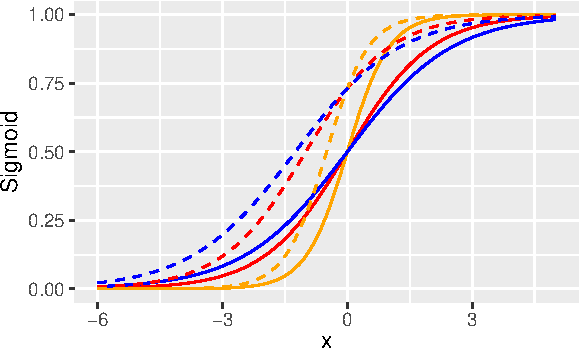
\includegraphics{L9_files/figure-beamer/unnamed-chunk-1-1.pdf}
\end{frame}

\begin{frame}
\textbf{Softmax} Showing \(K=3\) with
\(\frac{\exp{\beta_k x}}{\sum_{k=1}^3 \exp{\beta_{k} x }}\) where
\(\beta_1=1\) (red), \(\beta_2=1.1\) (orange) and \(\beta_3=0.9\)
(green).

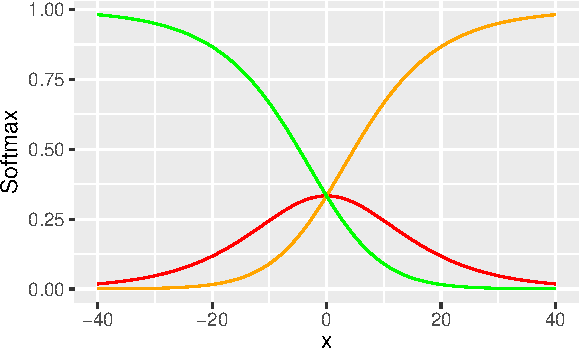
\includegraphics{L9_files/figure-beamer/unnamed-chunk-2-1.pdf}
\end{frame}

\begin{frame}
Observe that adding a constant what is in the exponent does not change
the function. Softmax has to be handled smart so that not overflow
(value in exponent too large) will be a problem, and that log(softmax)
is calculated in a numerically stable way. Many smart tricks starting at
page 21- in Slide deck from Ch 4 of Goodfellow, Bengio, and Courville
(2016)
\href{https://www.deeplearningbook.org/slides/04_numerical.pdf}{Numerical
precision: a deep learning super skill}
\end{frame}

\begin{frame}
\textbf{Softmax} Showing \(K=2\) with
\(\frac{\exp{\beta_k x}}{\sum_{k=1}^2 \exp{\beta_{k} x }}\) where
\(\beta_1=1\) (red), \(\beta_2=1.1\) (orange). Observe that this is that
same as using a sigmoid for one of the classes.

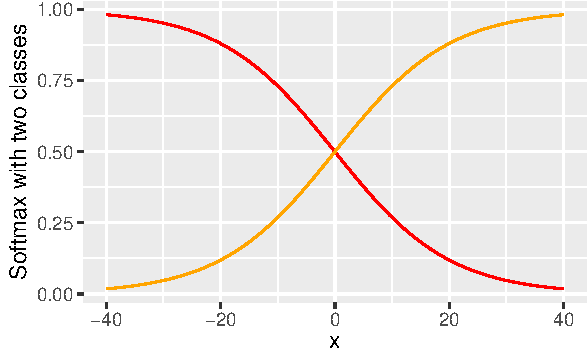
\includegraphics{L9_files/figure-beamer/unnamed-chunk-3-1.pdf}
\end{frame}

\begin{frame}
\begin{block}{Universal approximation property and hidden units}
\protect\hypertarget{universal-approximation-property-and-hidden-units}{}
\(~\)

\begin{itemize}
\tightlist
\item
  Remember: The goal is to \emph{approximate} some function \(f^*\) by
  \(f(x;\theta)\) - where both \emph{non-linearity} and
  \emph{interactions between covariates} are included.
\end{itemize}

\(~\)

\begin{itemize}
\tightlist
\item
  What type of mathematical function can a FFN with one hidden layer and
  linear output activation represent?
\end{itemize}

\(~\)
\end{block}
\end{frame}

\begin{frame}
The \emph{universal approximation theorem} says that a FFN with

\begin{itemize}
\tightlist
\item
  a \emph{linear output layer}
\item
  at least one hidden layer with a ``squashing'' activation function and
  ``enough'' hidden units
\end{itemize}

can approximate any (Borel measurable) function from one
finite-dimensional space (our input layer) to another (our output layer)
with any desired non-zero amount of error.

The theorem has been shown both for the sigmoid (logistic) and ReLU
activation functions in the hidden layer.
\end{frame}

\begin{frame}
Goodfellow, Bengio, and Courville (2016), page 198. See also Ripley
(1996) Ch 5.7 for a ``readable display.'' ELS Ch 11: universal
approximation is also true for a projection pursuit regression - which
in the 1990s was the statisticians ``competing solution'' for universal
approximation (not FNNs).
\end{frame}

\begin{frame}
\textbf{The rectified linear unit ReLU} \(\max(0,a)\) (90\% of all FNN)

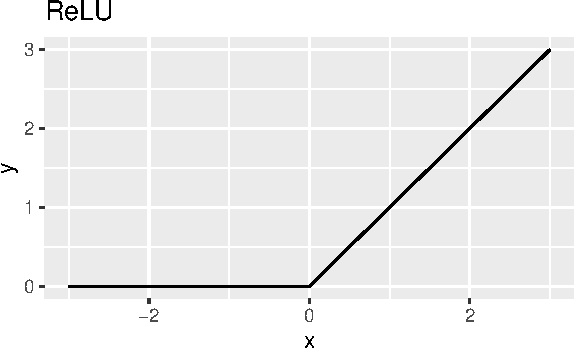
\includegraphics{L9_files/figure-beamer/unnamed-chunk-4-1.pdf}

The ReLU function is piecewise linear, but in total non-linear. Left
gradient 0 and right -1, with discontinuity of derivative at 0.
\end{frame}

\begin{frame}
Even though a large feedforward network with one hidden layer may be
able to represent a desired function, we may not be able to
\emph{estimate} the parameters of the function from training data,

\begin{itemize}
\tightlist
\item
  we may choose a too many or too few nodes in the hidden layer
\item
  our optimization routine may fail
\item
  we may overfit/underfit the training data
\end{itemize}

Therefore, sometimes networks with more than one hidden layer is used
--- with fewer total number of nodes but more layers. A network with
many hidden layers is called a \emph{deep network}.

\(~\)

\emph{Empirically, greater depth does seem to result in better
generalization for a wide variety of tasks.}

Goodfellow, Bengio, and Courville (2016) page 201.
\end{frame}

\begin{frame}
\begin{block}{Group discussion}
\protect\hypertarget{group-discussion}{}
(first two were given at the oral exam in 2019)

\begin{enumerate}
\item
  Why do we need to use non-linear activation functions when defining a
  neural network model?
\item
  One of the most popular activation function is called Rectified Linear
  Unit (ReLU), defined as \(g(x) = \max(x,0)\). What makes this
  activation function so attractive?
\item
  Solve this exam question from TMA4268V2019
\end{enumerate}

\textbf{a)} Which network architecture and activation functions does
this formula give? Include a drawing of the network architecture.

\[ \hat{y}({\bf x})=[1+\exp(-\beta_{01}-\sum_{m=1}^2 \beta_{m1}\max(\gamma_{0m}+\]
\[\sum_{l=1}^{3} \gamma_{lm}\max(\alpha_{0l}+\sum_{j=1}^{4}\alpha_{jl}x_j,0),0))]^{-1}\]
\textbf{b)} How many parameters are estimated in this network?

\textbf{c)} Which type of problem can this network be used to solve, and
what would you use as loss function?

\textbf{d)} Discuss briefly how parameters are estimated in a
feedforward neural network.
\end{block}
\end{frame}

\begin{frame}
\begin{block}{Additional exam questions from TMA4268V2019}
\protect\hypertarget{additional-exam-questions-from-tma4268v2019}{}
\textbf{a)} Write down the mathematical formula for a feedforward
network with one input layer, one hidden layer and one output layer,
with the following architecture

\begin{itemize}
\tightlist
\item
  input layer: seven input nodes and one bias node for the hidden layer,
\item
  hidden layer: four nodes, and a bias node for the output layer,
\item
  output layer: one node.
\end{itemize}

Let the nodes in the hidden layer have sigmoid activation function and
the node in the output layer have linear activation function.

A drawing of the network is provided.

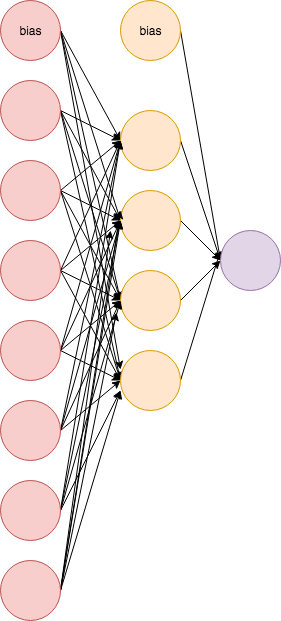
\includegraphics[width=300pt]{nn741}

\textbf{b)} Which type of problem can this network solve?

\textbf{c)} What would be an appropriate loss function (give
mathematical formula)?

Solutions to both exam problems are found here:
\url{https://www.math.ntnu.no/emner/TMA4268/Exam/e2019sol.html}
\end{block}
\end{frame}

\begin{frame}{Regularization}
\protect\hypertarget{regularization}{}
Goodfellow, Bengio, and Courville (2016), Chapter 7

\(~\)

\textbf{What:} any modification we make to a learning algorithm that is
intended to reduce its generalization (test) error but not its training
error.

\(~\)

\textbf{Or:} we need not focus entirely on finding the model of
``correct size'' (is that unique?), but instead find (too) a large model
that has been regularized properly.

\(~\)

In Part 1 (and 2) we wanted to construct a \emph{biased estimator} with
\emph{less variance} (than the unbiased estimator) so that the
\emph{bias-variance trade-off} gave a smaller expected loss on future
data, \(\text{Err}\), than for the unbiased estimator.
\end{frame}

\begin{frame}
\begin{block}{Penalization}
\protect\hypertarget{penalization}{}
Regularized loss (objective) function
\[\tilde{J}(\theta; {\bf X}, {\bf y})=J(\theta; {\bf X}, {\bf y})+\alpha \Omega(\theta)\]

\(~\)

\begin{itemize}
\tightlist
\item
  \({\bf X}, {\bf y}\) covariates and responses in training data.
\item
  Penalty parameter is now \(\alpha\) - previously \(\lambda\).
\end{itemize}

\(~\)

\begin{itemize}
\tightlist
\item
  As in Part 1 the bias term is not regularized - if done it may lead to
  underfitting. Notation: \(\theta\) for all parameters, but \({\bf w}\)
  for weights - and the bias \(b\) is then not a part of the weights.
\end{itemize}

\(~\)

\begin{itemize}
\tightlist
\item
  Different from Part 1: now the weights are not only for each input,
  but also for non-linearities in each input and interactions between
  the inputs. Why is that?
\end{itemize}

\(~\)
\end{block}
\end{frame}

\begin{frame}
\begin{block}{Weight decay}
\protect\hypertarget{weight-decay}{}
aka \(L_2\), ridge regression or Tikhonov regularization.

\[\Omega(\theta)=\frac{1}{2} {\bf w}^T {\bf w}\]

\textbf{Q:} Why are we penalizing towards 0, and not towards the true
value of the parameter?

\(~\)

In Wieringen (2020) we studied (briefly) the interpretation of the ridge
penalty for multiple linear regression, and will elaborate a bit more
here - and then relate to FNN.

\[ {\bf w}=({\bf X}^T{\bf X}+\alpha {\bf I})^{-1}{\bf X}^T{\bf y}\]
\end{block}
\end{frame}

\begin{frame}
Assume covariates and response are centered (no intercept needed). To
look at figures we let the number of covariates be \(p=2\), and assume
that both covariates contribute equally to the response (weigths without
penalization would be the same).

\(~\)

\begin{enumerate}
[1)]
\tightlist
\item
  Assume covariates are uncorrelated with the same variance, so that the
  estimated covariance matrix \(\frac{1}{n}{\bf X}^T{\bf X}\) is
  diagonal. Ridge: The weights for each covariate is then shrunken with
  the same factor.
\end{enumerate}

\(~\)

\begin{enumerate}
[1)]
\setcounter{enumi}{1}
\tightlist
\item
  Assume covariates are uncorrelated with different variances. Then the
  weights for the covariate with the largest variance is shrunken less
  than the covariate with the smallest variance (the weight for the
  covariate with the larger variance is larger than for the other).
\end{enumerate}

\(~\)
\end{frame}

\begin{frame}
Remark: if covariates are standardized the variances are the same. Then
ridge estimates before and after scaling will not simply differ by a
factor.
\end{frame}

\begin{frame}
\begin{figure}
\includegraphics[width=1\linewidth]{WNvWfig15bottom} \caption{Figure 1.5 of W. N. van Wieringen (2020)}\label{fig:unnamed-chunk-6}
\end{figure}
\end{frame}

\begin{frame}
\begin{enumerate}
[1)]
\setcounter{enumi}{2}
\tightlist
\item
  Assume covariates are correlated but have the same variance. The ridge
  shrinks less the weights of the strongly positively correlated
  covariates.
\end{enumerate}

\begin{figure}
\includegraphics[width=0.6\linewidth]{WNvWfig16left} \caption{Figure 1.6 of W. N. van Wieringen (2020)}\label{fig:unnamed-chunk-7}
\end{figure}
\end{frame}

\begin{frame}
In ELS (Ch 3.4.1) we looked at the singular value decomposition of the
covariate matrix \({\bf X}\), and the result was that:

\[\hat{y}_{\text{ridge}}={\bf X}\hat{\beta}_{\text ridge}= \cdots =
{\bf U}{\bf D}^2({\bf D}^2+\alpha {\bf I}_p)^{-1}{\bf U}^T {\bf y}=
\sum_{j=1}^p {\bf u}_j \frac{d_j^2}{d_j^2+\alpha}{\bf u}_j^T {\bf y}\]

\begin{itemize}
\tightlist
\item
  The estimated covariance matrix for centred covariates is
  \(\frac{1}{N}{\bf X}^T{\bf X}\). The eigenvalues of
  \({\bf X}^T{\bf X}\) are the squared singular values, \(d^2_j\).
\item
  The small singular values \(d_j\) correspond to directions in the
  column space of \({\bf X}\) with small variance, which will be the
  direction for the last principal components.
\end{itemize}

\(~\)

\begin{itemize}
\tightlist
\item
  The ridge penalties shrinks the direction with the small singular
  values the most. (Which is the same as we saw with the highly
  correlated directions being shrunken less.)
\end{itemize}

\(~\)
\end{frame}

\begin{frame}
In Goodfellow, Bengio, and Courville (2016), the transition over to FNN
is done by first looking at the effect of the penalty term in gradient
descent.

\begin{block}{Gradient descent}
\protect\hypertarget{gradient-descent}{}
Let \(\nabla J({\boldsymbol \theta}^{(t)})\) be the gradient of the loss
function evaluated at the current estimate
\({\boldsymbol \theta}^{(t)}\), then a step \(t+1\) of the algorithm the
new values (estimates) of of the parameters are given as:

\(~\)

\[{\boldsymbol \theta}^{(t+1)}={\boldsymbol \theta}^{(t)} - \epsilon \nabla_{\boldsymbol \theta} J({\boldsymbol \theta}^{(t)})\]

The \emph{learning rate} \(\epsilon\) is often set to some small value
(\(0.01\)).

\(~\)

The gradient is the vector of partial derivative of the loss function
with respect to each of the parameter in the network.

\(~\)
\end{block}
\end{frame}

\begin{frame}
\begin{block}{Effect of penalty on gradient}
\protect\hypertarget{effect-of-penalty-on-gradient}{}
Assume not bias parameter (maybe centering of covariates and response)

\[\tilde{J}({\bf w}; {\bf X}, {\bf y})=J({\bf w}; {\bf X}, {\bf y})+\frac{\alpha}{2}{\bf w}^T {\bf w}\]
\[\nabla_{\bf w} \tilde{J}({\bf w}; {\bf X}, {\bf y})=\nabla_{\bf w} J({\bf w}; {\bf X}, {\bf y})+\alpha{\bf w}\]
Gradient step with learning rate \(\epsilon\)

\[{\bf w}^{(t+1)}={\bf w}^{(t)}-\epsilon \cdot (\nabla_{\bf w} J({\bf w}^{(t)}; {\bf X}, {\bf y})+\alpha{\bf w}^{(t)})\]
\[{\bf w}^{(t+1)}=(1-\alpha \epsilon){\bf w}^{(t)}-\epsilon \cdot (\nabla_{\bf w} J({\bf w}^{(t)}; {\bf X}, {\bf y})\]

The effect is to shrink the weight be a constant factor at each step.

This is a local effect - on one gradient step.
\end{block}
\end{frame}

\begin{frame}
\begin{block}{Effect of penalty in quadratic approximation}
\protect\hypertarget{effect-of-penalty-in-quadratic-approximation}{}
\(~\)

For the multiple linear regression with quadratic loss the loss function
is also a quadratic function in the weights.

\(~\)

For a FNN with a general loss function we may use a quadratic
approximation close to the optimal weights
\({\bf w}^*=\text{argmin}_{\bf w} J({\bf w})\) from the unregularized
problem:

\begin{align*}\hat{J}({\bf w}; {\bf X}, {\bf y})&= J({\bf w}^*; {\bf X}, {\bf y})+\nabla_{\bf w} J({\bf w}^*; {\bf X}, {\bf y})({\bf w}-{\bf w}^*)\\
&+\frac{1}{2} ({\bf w}-{\bf w}^*){\bf H}_J({\bf w}-{\bf w}^*)
\end{align*}

where \(H_J\) is the Hessian matrix (matrix of partial second
derivatives) of the loss function \(J\) with respect to \({\bf w}\) and
evaluated at \({\bf w}^*\).
\end{block}
\end{frame}

\begin{frame}
\(~\)

Since \({\bf w}^*\) is a minimum of \(J\) then the gradient is (close
to) 0, and the Hessian should be positive semidefinite.

\(~\)

The gradient of the approximation is then
\[\nabla_{\bf w} \hat{J}({\bf w}; {\bf X}, {\bf y})={\bf H}_J({\bf w}-{\bf w}^*)\]
And setting the gradient equal \({\bf 0}\) shows that \({\bf w}^*\) is
the solution.

\(~\)

Adding the penalty term to the gradient approximation changes this:

\[\nabla_{\bf w} \tilde{\hat{J}}({\bf w}; {\bf X}, {\bf y})={\bf H}_J({\bf w}-{\bf w}^*)+\alpha {\bf w}\]
\end{frame}

\begin{frame}
Setting this equal to \({\bf 0}\) we call the new minimum
\(\tilde{\bf w}\)

\begin{eqnarray*}
{\bf 0}={\bf H}_J(\tilde{\bf w}-{\bf w}^*)+\alpha \tilde{\bf w}\\
({\bf H}_J(\tilde{\bf w}-\alpha {\bf I})\tilde{\bf w}={\bf H}{\bf w}^*\\
\tilde{\bf w}=({\bf H}+\alpha {\bf I})^{-1}{\bf H}{\bf w}^*
\end{eqnarray*}

Comparing this to the ridge regression solution
\[ {\bf w}=({\bf X}^T{\bf X}+\alpha {\bf I})^{-1}{\bf X}^T{\bf y}\] and
from Part 1 L2 (exercise) we saw that this can be written as

\[ {\bf w}^{\text ridge}=({\bf X}^T{\bf X}+\alpha {\bf I})^{-1}{\bf X}^T{\bf X}{\bf w}^{\text LS}\]

The difference is just that \({\bf X}^T {\bf X}\) for the ridge
regression is replaced by \({\bf H}\) for the quadratic approximation.
\end{frame}

\begin{frame}
For the GLM with canonical link the Hessian of the (negative)
log-likelihood is in general equal to the Fisher information matrix,
which is \({\bf H}={\bf X}^{T}{\bf W}{\bf X}\). Here \({\bf W}\) is a
diagonal matrix involving the derivative of the response function and
the variance of the response. For the normal case \({\bf W}\) is equal
\(\frac{1}{\sigma^2}\).

\(~\)

With the Hessian taking the place of the \({\bf X}^T{\bf X}\) in our
results from the ridge regression we may also now conclude that

\begin{itemize}
\tightlist
\item
  the ridge penalty shrinks the directions of the small eigenvalue of
  the Hessian matrix the most.
\end{itemize}

\(~\)

(Study Figure 7.1 in Goodfellow, Bengio, and Courville (2016).)
\end{frame}

\begin{frame}
\begin{block}{\(L_1\) penalty}
\protect\hypertarget{l_1-penalty}{}
\(~\)

\begin{itemize}
\tightlist
\item
  We know that it is hard to write solutions on closed form except for
  very special cases as for linear regression with orthogonal
  covariates.
\end{itemize}

\(~\)

\begin{itemize}
\tightlist
\item
  We saw from Part 1 that gradient methods were difficult for the lasso.
\end{itemize}

\(~\)

\begin{itemize}
\tightlist
\item
  Combinations of \(L_1\) and \(L_2\), elastic net, is also implemented
  for FNNs.
\end{itemize}

\(~\)
\end{block}
\end{frame}

\begin{frame}
\begin{block}{Early stopping}
\protect\hypertarget{early-stopping}{}
Goodfellow, Bengio, and Courville (2016), Ch 7.8.

The most commonly used for of regularization for FNN is \emph{early
stopping}.

\(~\)

\begin{itemize}
\tightlist
\item
  If we have chosen a sufficiently large model with the capacity to
  overfit the training data, we would observe that the training error
  decreases steadily during training, but the error on the validation
  set at some point begins to increase.
\end{itemize}

\(~\)

\begin{itemize}
\tightlist
\item
  If we stop the learning early and return the parameters giving the
  best performance on the validation set, this model would hopefully be
  a better model than if we trained the model until convergence --- and
  this model will then also give a better test set error.
\end{itemize}

\(~\)
\end{block}
\end{frame}

\begin{frame}
\begin{itemize}
\tightlist
\item
  It is possible to think of the number of \emph{training steps} as a
  hyperparameter. This hyperparameter can easily be set, and the cost is
  just that we need to monitor the performance on the validation set
  during training.
\end{itemize}

\(~\)

(Study figure 7.3 of Goodfellow, Bengio, and Courville (2016) for
U-shaped behaviour on validation set.)
\end{frame}

\begin{frame}
\(~\)

\begin{itemize}
\tightlist
\item
  Algo 7.1: For early stopping we need to save the weights as we train,
  then find the optimal point to stop the training - and then use the
  weights from that point in the training.
\end{itemize}

\(~\)

\begin{itemize}
\tightlist
\item
  Algo 7.2: First find the optimal stopping time for the training based
  on the validation set, and then retrain the full training set
  (including the validation part) and stop at the selected stopping
  time. (Algo 7.2)
\end{itemize}

\(~\)

\begin{itemize}
\tightlist
\item
  Algo 7.3: Start from the weight of Algo 7.3, and continue training but
  now with the full training set. Even though the validation set is now
  a part of the training scheme, monitor the average performance on the
  validation set and stop when the performance goes below the value of
  the training set objective when the early stopping stopped. This
  strategy may not be optimal or even terminate.
\end{itemize}
\end{frame}

\begin{frame}
\(~\)

\begin{itemize}
\tightlist
\item
  Why is early stopping a regularization technique? By early stopping
  the optimization procedure has only seen a relatively small part of
  the parameter space in the neighbourhood of the initial parameter
  value.
\end{itemize}

\(~\)

\begin{itemize}
\tightlist
\item
  There is a formal equivalence between early stopping and \(L_2\)
  regularization for a linear regression and squared loss, elaborating
  on the trajectory of the gradient descent during training.
\end{itemize}

\textbf{Q: Should details on the result be included?}

\(~\)

(Study figure 7.4 of Goodfellow, Bengio, and Courville (2016) for a
comparison with \(L_2\) regularization.)
\end{frame}

\begin{frame}
\begin{block}{Bagging and ensembles}
\protect\hypertarget{bagging-and-ensembles}{}
Goodfellow, Bengio, and Courville (2016) Ch 7.7

\(~\)

\begin{itemize}
\tightlist
\item
  FNN are also suitable for making ensembles - for example by just
  averaging predictions from many runs of optimization - so no
  bootstrapping.
\end{itemize}

\(~\)

\begin{itemize}
\tightlist
\item
  Here the FFNs then are trained

  \begin{itemize}
  \tightlist
  \item
    from different random initializations
  \item
    random selections of minibatches
  \item
    different hyperparameters
  \end{itemize}
\end{itemize}

\(~\)
\end{block}
\end{frame}

\begin{frame}
\begin{block}{Dropout}
\protect\hypertarget{dropout}{}
(Goodfellow, Bengio, and Courville (2016), Section 7.12, Chollet and
Allaire (2018) 4.4.3) and will discuss more in L11.

Dropout was developed by Geoff Hinton and his students.

\begin{itemize}
\tightlist
\item
  During training: randomly \emph{dropout} (set to zero) outputs in a
  layer. Drop-out rates may be chosen between 0.2 and 0.5.
\item
  During test: not dropout, but scale done the layer output values by a
  factor equal to the drop-out rate (since now more units are active
  than we had during training)
\end{itemize}

Alternatively, the drop-out and scaling (now upscaling) can be done
during training.
\end{block}
\end{frame}

\begin{frame}
One way to look at dropout is on the lines of what we did in Module 8
when we used bootstrapping to produced many data sets and then fitted a
model to each of them and then took the average (bagging). But randomly
dropping out outputs in a layer, this can be looked as mimicking bagging
--- in an efficient way.

See Goodfellow, Bengio, and Courville (2016), Section 7.12 for more
insight into the mathematics behind drop-out, and we will look more into
drop-out in L11.

\textbf{some QC remaining}
\end{frame}

\begin{frame}
\begin{block}{Group discussion}
\protect\hypertarget{group-discussion-1}{}
(first was asked at the oral exam in 2019)

\begin{enumerate}
[1)]
\item
  Can you mention three different techniques to prevent overfitting?
  What are key aspects of one of the techniques? Have you used any of
  theses yourself? Elaborate.
\item
  Which courses (or self study?) have you done to learn about neural
  networks? What is the most interesting aspect of neural network (your
  opinion)?
\item
  What is your experience with using Python or R to fit (deep) FNN?
  ``Packages'' used?
\item
  What is the connection between an artificial neural network and the
  neural network of our brains (that is studied in the field of
  neuroscience)?
\end{enumerate}

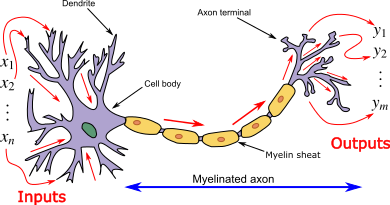
\includegraphics[width=500pt]{./Neuron3}

Image title: Neuron and myelinated axon, with signal flow from inputs at
dendrites to outputs at axon terminals. Image credits: By Egm4313.s12
(Prof.~Loc Vu-Quoc) - Own work, CC BY-SA 4.0,
\url{https://commons.wikimedia.org/w/index.php?curid=72816083}
\end{block}
\end{frame}

\begin{frame}{Optimization}
\protect\hypertarget{optimization}{}
\begin{block}{Gradient descent}
\protect\hypertarget{gradient-descent-1}{}
Explained above.
\end{block}

\begin{block}{Mini-batch stochastic gradient descent (SGD)}
\protect\hypertarget{mini-batch-stochastic-gradient-descent-sgd}{}
Goodfellow, Bengio, and Courville (2016) Ch 8.3.1

The loss function is computed as a mean over all training examples.

\[J({\boldsymbol \theta})=\frac{1}{n}\sum_{i=1}^n J({\bf x}_i, y_i)\]

This means that the gradient will also be a mean over the gradient
contribution from each training example.

\[\nabla_{\boldsymbol \theta} J({\boldsymbol \theta})=\frac{1}{n}\sum_{i=1}^n \nabla_{\boldsymbol \theta} J({\bf x}_i, y_i)\]
\end{block}
\end{frame}

\begin{frame}
To build a network that generalizes well, it is important to have many
training examples, but that would make us spend a lot of time and
computer resources at calculating each gradient descent step.

We observe that we may see the gradient as an average over many
individual gradients, and think of this as an estimator for an
expectation. This expectation can we (also) approximate by the average
gradient over just a \emph{mini-batch} (random sample) of the
observations.

The idea here is that the optimizer will converge much faster if they
can rapidly compute approximate estimates of the gradient, instead of
slowly computing the exact gradient (using all training data).

In addition with multicore systems, mini-batches may be processed in
parallell and the batch size is often a power of 2 (32 or 256).

It also turns out that small batches also serves as a regularization
effect maybe due to the variability they bring to the optimization
process.
\end{frame}

\begin{frame}
In the 4th video (on backpropagation) from 3Blue1Brown there is nice
example of one trajectory from gradient decent and one from SGD (13:50
minutes into the video):
\url{https://www.youtube.com/watch?v=tIeHLnjs5U8}
\end{frame}

\begin{frame}
This means that for (mini-batch) stochastic gradient descent we do as
follows:

\begin{enumerate}
\tightlist
\item
  Divide all the training samples randomly into mini-batches.
\item
  For each mini-batch: Make predictions of the reponses in the
  mini-batch in a \emph{forward pass}.
\item
  Compute the loss for the training data in this batch.
\item
  Compute the gradient of the loss with regard to the model's parameters
  (\emph{backward pass}) based on the training data in the batch.
  \(\nabla_{\boldsymbol \theta}^* J({\boldsymbol \theta}^{(t)})\)
\item
  Update all weighs, but just using the average gradient from the
  mini-batch
  \({\boldsymbol \theta}^{(t+1)}={\boldsymbol \theta}^{(t)} - \lambda \nabla_{\boldsymbol \theta} ^* J({\boldsymbol \theta}^{(t)})\)
\item
  Repeat 2-5 until convergence. (Could have gone back to 1, but often
  not done.)
\end{enumerate}
\end{frame}

\begin{frame}
\begin{itemize}
\tightlist
\item
  The algorithm defined above is called mini-batch SGD. The Stochastic
  part comes from the fact that we are randomly sampling batches from
  the training data.
\item
  Stochastic gradient descent (SGD) for size equals to 1.
\item
  Mini-batch SGD is a compromise between SGD (one sample per iteration)
  and full gradient descent (full dataset per iteration)
\end{itemize}
\end{frame}

\begin{frame}
\begin{block}{Backpropagation algorithm}
\protect\hypertarget{backpropagation-algorithm}{}
Computing the analytical expression for the gradient \(\nabla J\) is not
difficult, but the numerical evaluation may be expensive. The
Backpropagation algorithm is an simple and inexpensive way to calculate
the gradient.

The chain rue is used to compute derivatives of functions of other
functions where the derivatives are known, this is done efficiently with
backpropagation.

Backpropagation starts with the value of the loss function and works
backward from the top layers to the bottom layers, applying the chain
rule to compute the contribution that each parameter have in the loss
value.
\end{block}
\end{frame}

\begin{frame}
More information:

\begin{itemize}
\tightlist
\item
  Mathematical details in Goodfellow, Bengio, and Courville (2016)
  Section 6.5 (pages 204-238),
\item
  3Blue1Brown: video overview:
  \url{https://www.youtube.com/watch?v=Ilg3gGewQ5U} and chain rule maths
  \url{https://www.youtube.com/watch?v=tIeHLnjs5U8}
\end{itemize}
\end{frame}

\begin{frame}[fragile]
\begin{block}{Variations of SDG --- with adaptive learning rates}
\protect\hypertarget{variations-of-sdg-with-adaptive-learning-rates}{}
Goodfellow, Bengio, and Courville (2016) 8.5

General concept:

\begin{itemize}
\tightlist
\item
  momentum term: previous gradients are allowed to contribute.
\end{itemize}

Named variants: In \texttt{keras} the ``default optimizer'' is RMSprop.

\begin{itemize}
\tightlist
\item
  AdaGrad: individually adapt the learning rates of all model parameters
  by scaling them inversely proportional to the square root of the sum
  of all their historical squared values. (Nice properties for convex
  problems, but with non-linear hidden activation function we do not
  have a convex problem.)
\item
  RMSprop: modification to AdaGrad in non-convex setting. Scales with
  exponentially weighted moving average instead of all historical
  squared gradient values.
\end{itemize}
\end{block}
\end{frame}

\begin{frame}
\begin{block}{Further reading on optimizers}
\protect\hypertarget{further-reading-on-optimizers}{}
\begin{itemize}
\tightlist
\item
  \href{https://keras.io/optimizers/}{Keras documentation for
  Optimizers}
\item
  \href{http://ruder.io/optimizing-gradient-descent/index.html}{An
  overview of gradient descent optimization algorithms}
\item
  \href{http://www.cs.toronto.edu/~tijmen/csc321/slides/lecture_slides_lec6.pdf}{Overview
  of mini-batch gradient descent}
\item
  Andrew Ng explains about RMSprop in Coursera course:
  \href{https://www.coursera.org/learn/deep-neural-network/lecture/BhJlm/rmsprop}{Improving
  Deep Neural Networks: Hyperparameter tuning, Regularization and
  Optimization}
\end{itemize}
\end{block}
\end{frame}

\begin{frame}{Keras in R}
\protect\hypertarget{keras-in-r}{}
\begin{itemize}
\tightlist
\item
  \url{https://keras.rstudio.com/}
\item
  Cheat-sheet for R Keras:
  \url{https://github.com/rstudio/cheatsheets/raw/master/keras.pdf}
\item
  \href{https://keras.io/optimizers/}{Keras documentation for
  Optimizers}
\end{itemize}

\begin{block}{Resources from MA8701 in 2019}
\protect\hypertarget{resources-from-ma8701-in-2019}{}
(made by Thiago G. Martins)

All files:
\url{https://www.math.ntnu.no/emner/MA8701/2019v/DeepLearning/}

And with focus on running Keras:

\begin{itemize}
\tightlist
\item
  What is and installing:
  \url{https://www.math.ntnu.no/emner/MA8701/2019v/DeepLearning/3-keras.html}
\item
  Setting up model:
  \url{https://www.math.ntnu.no/emner/MA8701/2019v/DeepLearning/4-deep_learning_models.html}
\item
  Compiling:
  \url{https://www.math.ntnu.no/emner/MA8701/2019v/DeepLearning/5-compiling_deep_learning_models.html}
\item
  Overfitting (regularization and dropout)
  \url{https://www.math.ntnu.no/emner/MA8701/2019v/DeepLearning/7-prevent_overfitting.html}
\item
  Boston housing:
  \url{https://www.math.ntnu.no/emner/MA8701/2019v/DeepLearning/11-neural_networks_boston_housing.html}
\end{itemize}

Thiago also has resources for analysing text (with IMBD data) and images
(with MNIST) at
\url{https://www.math.ntnu.no/emner/MA8701/2019v/DeepLearning/}, but for
the text analysis lecture we will use Python with sklearn and pyTorch.
\end{block}
\end{frame}

\begin{frame}{References and further reading}
\protect\hypertarget{references-and-further-reading}{}
\begin{itemize}
\tightlist
\item
  \href{https://www.math.ntnu.no/emner/TMA4268/2019v/11Nnet/11Nnet.html}{Introduction
  to artificial neural networks from TMA4268 in 2019}
\item
  \url{https://youtu.be/aircAruvnKk} from 3BLUE1BROWN - 4 videos - using
  the MNIST-data set as the running example
\item
  Explaining backpropagation
  \url{http://neuralnetworksanddeeplearning.com/chap2.html}
\item
  Look at how the hidden layer behave:
  \url{https://playground.tensorflow.org}
\item
  Friedman, Hastie, and Tibshirani (2001),Chapter 11: Neural Networks
\item
  Efron and Hastie (2016), Chapter 18: Neural Networks and Deep Learning
\end{itemize}

\hypertarget{refs}{}
\begin{CSLReferences}{1}{0}
\leavevmode\hypertarget{ref-kerasR}{}%
Chollet, François, and J. J. Allaire. 2018. \emph{Deep Learning with r}.
Manning Press.

\leavevmode\hypertarget{ref-casi}{}%
Efron, Bradley, and Trevor Hastie. 2016. \emph{Computer Age Statistical
Inference - Algorithms, Evidence, and Data Science}. Cambridge
University Press.

\leavevmode\hypertarget{ref-ESL}{}%
Friedman, Jerome, Trevor Hastie, and Robert Tibshirani. 2001. \emph{The
Elements of Statistical Learning}. Vol. 1. Springer series in statistics
New York.

\leavevmode\hypertarget{ref-goodfellow}{}%
Goodfellow, Ian, Yoshua Bengio, and Aaron Courville. 2016. \emph{Deep
Learning}. MIT Press.

\leavevmode\hypertarget{ref-ISL}{}%
James, Gareth, Daniela Witten, Trevor Hastie, and Robert Tibshirani.
2013. \emph{An Introduction to Statistical Learning}. Vol. 112.
Springer.

\leavevmode\hypertarget{ref-Ripley}{}%
Ripley, Brian D. 1996. \emph{Pattern Recognicion and Neural Networks}.
Cambridge University Press.

\leavevmode\hypertarget{ref-MASS}{}%
Venables, W. N., and B. D. Ripley. 2002. \emph{Modern Applied Statistics
with s}. Springer.

\leavevmode\hypertarget{ref-WNvW}{}%
Wieringen, Wessel N. van. 2020. {``Lecture Notes on Ridge Regression.''}
\url{https://arxiv.org/pdf/1509.09169.pdf}.

\end{CSLReferences}
\end{frame}

\end{document}
